\documentclass[10pt,a4paper,notitlepage]{report}
\usepackage[utf8]{inputenc}
\usepackage[english]{babel}
\usepackage{amsmath}
\usepackage{amsfonts}
\usepackage{amssymb}
\usepackage{hyperref}
\usepackage{graphicx}
\usepackage{listings}
\usepackage{lmodern}
\usepackage{fourier}
\usepackage[left=2cm,right=2cm,top=2cm,bottom=2cm]{geometry}
\author{Christopher Smith}
\title{Using ROS/Gazebo Simulator with SITL}
\begin{document}
\maketitle
\section*{Intro}
\noindent \textbf{DISCLAIMER:} This installation walkthrough and the software is owed to the hard work and efforts of the Ardupilot group and alexbuyval at Github and Bitbucket.\\

\noindent These instructions can be found at \hspace{2mm} \url{http://dev.ardupilot.com/wiki/using-rosgazebo-simulator-with-sitl}\\

\section*{LINUX INSTALL: Ubuntu 14.04}

\noindent \textbf{install-ros.bash}: Contains the installs for all the dependencies of the simulation.\\
\noindent \textbf{setup-ardu-workspace.bash}: Will create a workspace from the current directory for the simulation.\\

\noindent \textbf{IF YOU DO NOT WANT TO USE THE SCRIPTS}, you can copy and paste from the files to execute all or the portion of the script needed. The scripts do make life a bit easier.\\
\begin{enumerate}
\item Download the bash scripts found in this folder named \textit{install-ros.bash} and \textit{setup-ardu-workspace.bash}.
\item Make both files executable:
\begin{lstlisting}[language=bash]
$ chmod +x filename
\end{lstlisting}
\item Run both scripts sequentially. 
\begin{lstlisting}[language=bash]
$ ./install-ros.bash
$ ./setup-ardu-workspace.bash
\end{lstlisting}
\item Run the following command.
\begin{lstlisting}[language=bash]
$ export PATH=\$PATH:\$HOME/ardupilot/Tools/autotest 
\end{lstlisting}
Note: Use your own path to ardupilot folder in the line above!
\item You are done with the setup. You can begin using the simulation(Fig.~\ref{fig:sim}).
\end{enumerate}
\noindent \textbf{Installation Issues} If there are compilation issues using either catkin_make or catkin build then more packages will need to be installed using sudo apt-get install. It will usually be missing a config file for a library that will need to be installed.

\section*{Running the Simulation}

\begin{figure}[h]
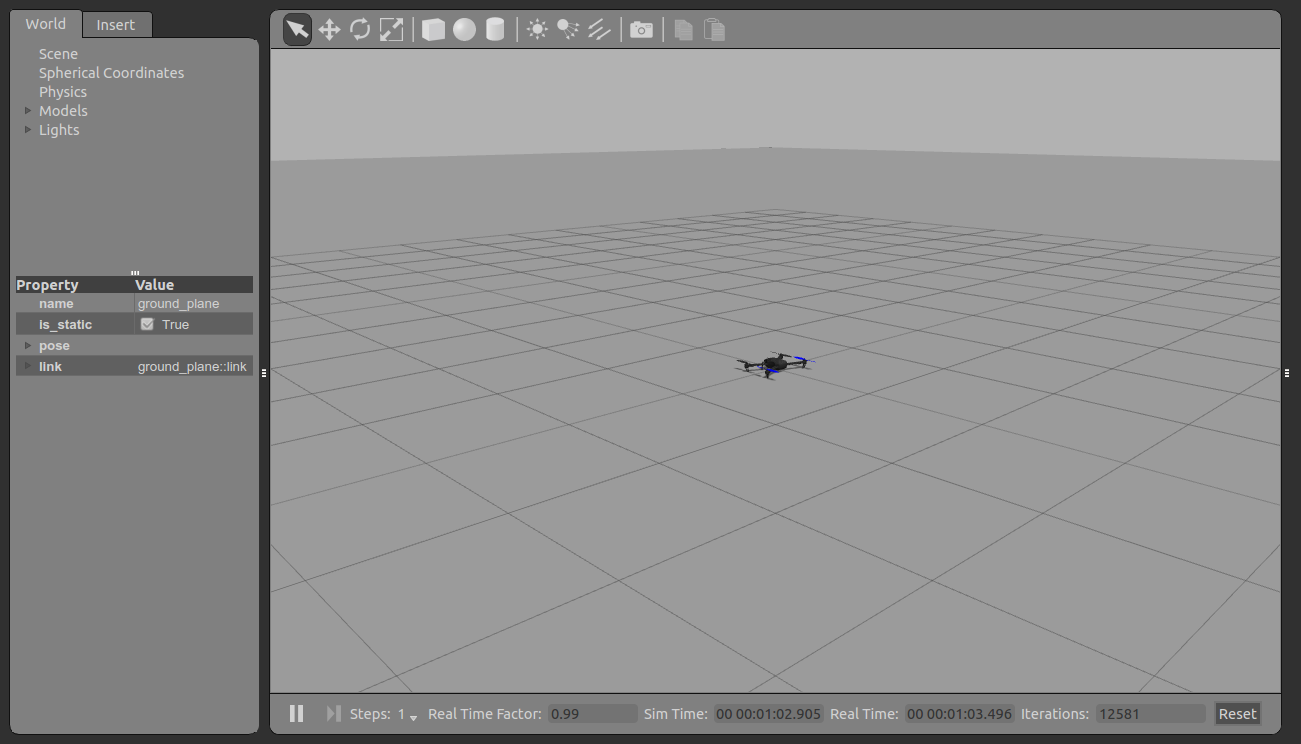
\includegraphics[width=4in]{rossitl.png}
\caption{UAV in Gazebo}
\label{fig:sim}
\end{figure}
\begin{enumerate}
\item Source the simulation
\begin{lstlisting}[language=bash]
your_workspace$ source devel/setup.bash 
\end{lstlisting}
\item Open a terminal and execute the script:
\begin{lstlisting}[language=bash]
$ cd ~/ardupilot/ArduCopter
$ sim_vehicle.sh -f arducopter_sitl_ros --console
\end{lstlisting}

\item At this point you can control the UAV with a specific controller. However modifying a config file will allow you to control the UAV manually using an XBox(or compatible) controller. We have found that other controllers are capable of controlling the craft, but the controls for steering and motor speed are mapped on the same stick.
\end{enumerate}


\noindent As a result of the flight controller being implemented using the ROS framework, the flight controller message traffic can be monitored using ROS tools(Fig.~\ref{fig:rostopics}), such as using:
\begin{lstlisting}[language=bash]
$ rosrun rqt_graph rqt_graph
\end{lstlisting}

\begin{figure}[h]
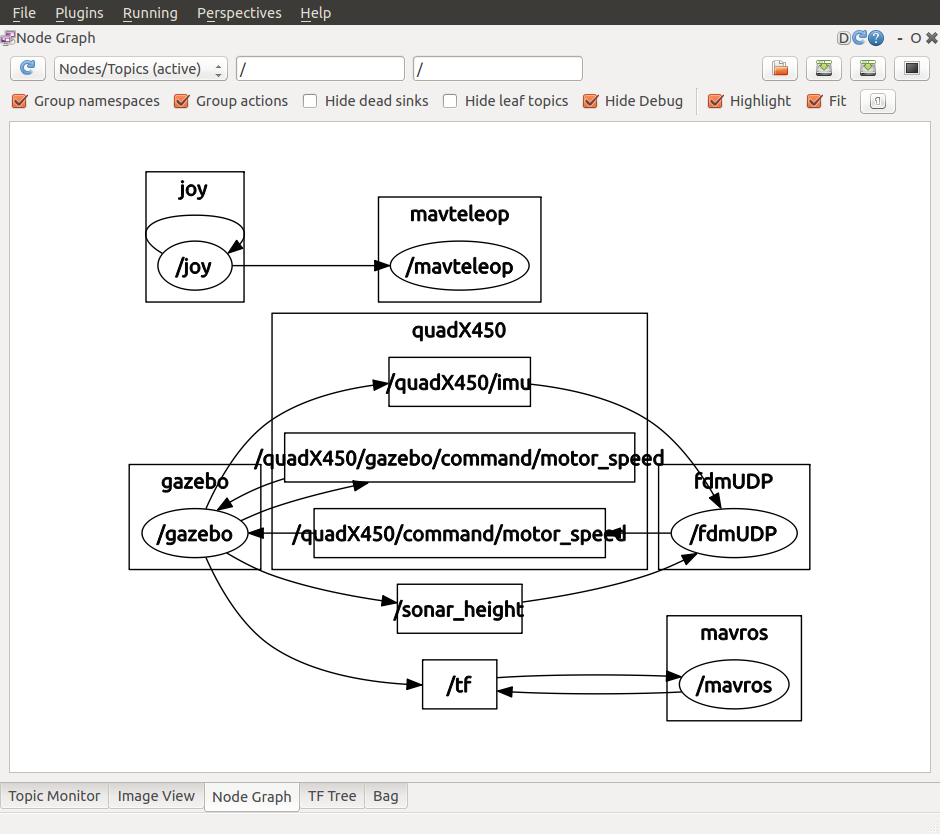
\includegraphics[scale=.35]{ardusitl.png}
\caption{ROS Topic Publishers and Subscribers}
\label{fig:rostopics}
\end{figure}


\end{document}